\documentclass[a4paper,twocolumn,twoside,10pt]{article}
\usepackage{graphicx,amsmath,amssymb,amsthm,subfig}

\makeatletter \oddsidemargin-.25in \evensidemargin-.25in
\makeatother \topmargin-0.75in \textwidth7in \textheight9.5in

\makeatletter

\newcommand{\noun}[1]{\textsc{#1}}



\makeatother


\markboth{$~$ \hfill {\rm\noun{A. Banos}, \noun{R. Doursat} and  \noun{ J. Raimbault}} \hfill $~$} {$~$ \hfill
{\rm Urban Configuration Optimization} \hfill$~$}

\pagestyle{myheadings} 


\begin{document}
\def \thepage {}
\date{}

% Title----------------------------------------------------------------
\title{\begin{flushleft}
\noindent {\small {\it Proceedings of ICCSA 2014
\\Normandie University, Le Havre, France - June 23-26, 2014\\[5mm]
 }}
\end{flushleft}\Large\bf \uppercase{Generative coupled model for Urban configuration optimization} }

\author{ \noun{A. Banos}, \noun{R. Doursat} and  \noun{ J. Raimbault}
 \thanks{\noun{A. Banos} is with G\'eographie-Cit\'es, UMR-CNRS 8504, Paris . E-mail:
arnaud.banos@parisgeo.cnrs.fr}
 \thanks{\noun{R. Doursat} is with School of Biomedical Engineering,
   Science and Health Systems, Drexel University, USA. E-mail:
rene.doursat@drexel.edu}
 \thanks{\noun{J. Raimbault} is with Graduate School, Ecole
   Polytechnique, France and LVMT, Ecole Nationale des Ponts et
   Chauss\'ees, France. E-mail:
juste.raimbault@polytechnique.edu}
\thanks{Manuscript received March 18, 2014}\\[20mm]}

 \maketitle



% Abstract----------------------------------------------------------------


{\footnotesize \noindent {\bf Abstract.}  We describe an hybrid agent-based model coupling a cellular automata
and a dynamic network, for the simulation of urban growth. Heterogeneous
aspects of urban systems are taken into account in the sense that
morphologic structure but also functional properties of the city are
implied in the evolution. Classic measures of description and performances
for generated configuration are used to classify and explore generated
patterns, and we also propose an economic evaluation of the structure
using sensitivity of segregation models to spatial configuration.
We can apply the model to a real-world situation, proposing an optimization
of the repartition of activities in a zoning context. \\
{\bf Keywords.} Agent-based modeling, Cellular automata, Bi-objective
Pareto optimization, Evidence-based urbanism, Urban morphogenesis.}




\section{Introduction}

Recent progress in many disciplines linked directly or indirectly
to Urban Planning can be interpreted as the development of a ``new
urban science'' as \noun{Batty} states in \cite{batty2013new}. From
agent-based modeling in quantitative geography, which achievements
are reviewed in \cite{heppenstall2012agent}, and for which the best
example of promising results are the series of Simpop models (\cite{pumain2012multi}),
to other approaches of the field that \noun{Portugali} present as
``Complexity theories of cities'' (\cite{portugali2012book}) that
can involve scientists such as physicists as \noun{Haken} on information
theory (\cite{haken2003face}) or architects as \noun{Hillier} with
Space Syntax theory (\cite{hillier1976space}), the field is broad
but is strongly consistent through the common view of urban systems
as complex systems.

In that context, Cellular Automata models (CA), in which agents (cells)
are fixed and evolve according to the state of neighbor cells, have
been broadly studied and used. Their use in urban planning, for reproduction
of existing urban forms and land-use patterns, was already described
by \noun{White} and \noun{Engelen} in \cite{white1993cellular} and
was later analysed (\cite{batty1997cellular,batty1997possible}) and
synthesized (\cite{Bat07}) by \noun{Batty. }A recent review of possible
application of CA models is done in \cite{iltanen2012cellular}. The
possible variations of models types and applications is quite broad
. For example, a microeconomic CA for simulation of sprawl is developed
in \cite{DBM11}. Measures for sustainable development of a fast growing
region in China are investigated in \cite{Wu96alinguistic} through
a ``linguistic'' CA, that is that the rule are in real time updated
thanks to interactions with the real population. Land-use modeling
approaches are one essential point, as was the first CA model by \noun{White}
. The two-dimensionnal aspect of the automaton is not mandatory,
as the example of the 1D CA model proposed in \cite{peeters2009space}
that allows to show discontinuities in settlement patterns and the
strong path-dependence of these. We propose to build a model in the
frame of CA modeling of urban systems.

Our model is adapted from the work of \noun{Moreno} \& \textit{al}.
(\cite{MBB09,moreno2007conception}), that proposed to integrate network
effects in a CA model for modeling urban morphology. Their aim was
to test the effects of physical proximity on urban shape, introducing
the modeling of urban mobility through a network whose evolution is
coupled with the evolution of the urban shape. We generalize the model,
allowing to take into account functional properties of the urban environment.
The concept of considering heterogeneous urban activities was introduced
in \cite{white2006modeling} and developed in \cite{van2012activity},
but was at our knowledge never considered from the point of view of
physical accessibility and the impact on sprawl patterns.

We describe formally the model in a first section and detail the
indicator functions used to quantify the generated patterns. We then propose internal and
external validations by sensitivity analysis and reproduction of
typical urban patterns. We are then able to apply the model to a
concrete case, proposing an bi-objective optimization heuristic for
functional configuration, with objective functions relevant indicators
that we have studied in the validation section.


\section{Model description}


\subsection{Agents and rules}

The world is a square lattice $(L_{i,j})_{1\leq i,j\leq N}$ constituted
of cells that can be occupied or not (that will be denoted by a function
$\delta(i,j,t)$, time being defined on a standard time scale $\mathbb{T}$
which definition is introduced in \cite{golden2012modeling}, and
for which we will take $\tau\mathbb{N}$, $\tau>0$ to simplify).
Among these fixed agents evolves an euclidian network whose agents
are roads: $N(t)=(V(t),E(t))$ whith $V$ finite part of the world
(set of points). At initial time, no cell is occupied and the initial
network is fixed: $N(0)=(V_{0},E_{0})$. In order to translate functional
mechanisms in the growth of the city, we suppose that a part of initial
nodes are city centers $C_{0}$ for each an activity is defined by
an integer-valued function $a:C_{0}\rightarrow\{1,\ldots,a_{max}\}$.
The initial network and centers can be either generated at random
(following consistent specifications) or following a user-defined
configuration.

In all generality, we suppose that there exists a fixed number of
functions defined on cells and in time, that we call explicative variables,
noted $(d_{k})_{1\leq k\leq K}$. Corresponding weights $(c_{k})_{1\leq k\leq K}\in[0,1]^{K}$
are parameters of the model. These will determine the value of cells
$v(i,j,t)$. In practice, these variables will be: $d_{1}$ the density
in a neighborhood of radius $r$ (parameter) around the cell; $d_{2}$
the distance to the nearest road; $d_{3}$ the distance to the nearest
town center through the network; and $d_{4}$ the ``accessibility''
of activities, defined as, with $d_{A}(a)$ distance to nearest center
with activity $a$ through the network, and $p_{A}\in[1;+\infty[$,
$d_{4}=\left\Vert (d_{A}(a))_{1\leq a\leq a_{max}}\right\Vert _{p_{A}}=\left(\frac{1}{a_{max}}\cdot\sum_{a=1}^{a_{max}}d_{A}(a)^{p_{A}}\right)^{1/p_{A}}$.

Giving these settings and variables, the evolution of the system for
one time step is the following:
\begin{itemize}
\item New cell values are calculated by $v(i,j,t)=\frac{1}{\sum_{k=1}^{K}c_{k}}\cdot\sum_{k=1}^{K}c_{k}\cdot\frac{(d_{k}^{max}-d_{k})}{(d_{k}^{max}-d_{k}^{min})}$.
It corresponds to a weighted average of the normalized heterogeneous
functions $d_{k}$, for which each influence is controlled by the
weight $c_{k}$.
\item $N$ new cells chosen as the $N$ cells with the best value are built
in a random order.
\item For each new cell built, if $d_{2}>d_{s}$ fixed parameter (distance
over which a new road is needed), the cell is connected to the network
by a new road connecting perpendicularly with the network
\end{itemize}
Note that the process is stochastic since it depends on the random
order on which the new cell are built. Sensitivity analysis and explorations
will determine the influence of respective parameters and the influence
of that stochastic aspect. The growth is stopped after a fixed amount
of time fixed by experience, so the final structure does not fill
totally the world, what would make no sense. A good compromise has
to be taken between ``unfinished'' structures and stationary result
totally biased by bord-effects.

Figure 1 shows a ``flowchart'' describing the working of the agent-based
model, especially what are the feedbacks between agents.



\begin{figure}[htp]
\centering
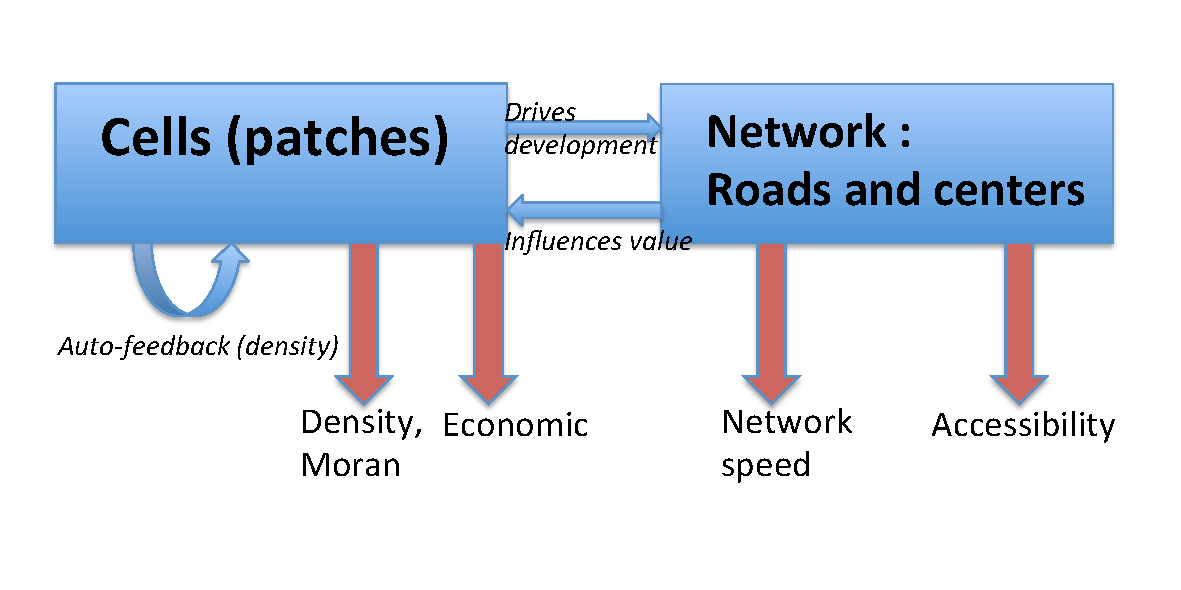
\includegraphics[width=0.45\textwidth]{figures/flowchart}
\caption{Flowchart of the model. Blue arrows represent interactions and feedbacks, whereas red arrows
are evaluation functions.}

\label{fig1}

\end{figure}




\subsection{Evaluation functions}

Once a structure has been generated, one need to quantify its properties,
either to classify it, or to compare it to other structures in an
optimization purpose. Therefore we need evaluation functions, that
can be both objective quantifications or fitness functions for structures.
The following proposed measures take into account all explicative
variables, since their distribution that is an emerging feature is
not supposed to be known before development and are therefore essential
to monitor, at the exception of the distance to roads ($d_{2}$) on
which we keep always control precisely because of the network development
rule (fixed distance $d_{s}$ over which a road is built).


\paragraph{Morphology}

We qualify the morphologic structure of a configuration by projecting
on a plane corresponding to the following indicators:
\begin{itemize}
\item The integrated local density, calculated by integration with a norm-p
of the densities in circular neighborhood of each cell (with same
radius parameter as for the run). We have, with $p_{d}\in[1;+\infty[$
\[
D(t)=\left[\frac{1}{\sum_{i,j}\delta(i,j,t)}\cdot\sum_{\delta(i,j,t)\neq0}d_{1}(i,j,t)^{p_{d}}\right]^{1/p_{d}}
\]

\item The Moran index, defined in \cite{tsai2005quantifying} and used a
lot in quantitative geography such as in \cite{lenechet:hal-00696445},
is used to quantify the polycentric character of the distribution
of populated cells. It takes values between -1 and 1, a value close
to 1 corresponding to a strong monocentric distribution, zero is for
totally random distribution and -1 for a ``chessboard-like'' distribution
(one cell over two is occupied). Polycentric distribution will have
small positives values according to the size and respective distance
of centers. The space is decomposed into $M$ regular areas (a grid
in practice, which size has to be at the intermediate scale between
cell size and world size, that is roughly $1\ll M\ll N$), and we
denote by $(P_{i})_{1\leq i\leq M}$ the occupied cells in each area
and $d_{ij}$ the distance between centroids of $i$ and $j$. The
Moran index of spatial auto-correlation is defined as
\end{itemize}
\[
M(t)=\frac{M}{\sum_{i\neq j}\frac{1}{d_{ij}}}\cdot\frac{\sum_{i\neq j}\frac{1}{d_{ij}}\cdot(P_{i}-\bar{P})(P_{j}-\bar{P})}{(\sum_{i=1}^{M}(P_{i}-\bar{P}))^{2}}
\]


We recognize the normalized ratio between a modified covariance (weighting
the pairwise correlations by the distance between centroids) and the
variance of the distribution.


\paragraph{Network performance}

Because of the way it evolves, the only loops in the network are the
initial ones. Therefore, it has no sense to evaluate robustness or
clustering coefficient of the network. However, since the generated
network is supposed to simulate the mobility network, we can evaluate
as suggested in \cite{banos2012towards} its performance through its
relative speed, i. e. the quantity of detours it obliges to make.
We define it, considering ony travels from occupied patches to nearest
center, with $p_{n}\in[1;+\infty[$, $d(ij,c)$ the euclidian distance
and $c_{min}^{ij}=argmin_{c\in C_{0}}(d_{ij\rightarrow c})$,

\[
S(t)=\left[\frac{1}{\sum_{i,j}\delta(i,j,t)}\cdot\sum_{\delta(i,j,t)\neq0}\left(\frac{d_{3}(i,j,t)}{d(ij,c_{min}^{ij})}\right)^{p_{n}}\right]^{1/p_{n}}
\]



\paragraph{Functional accessibility}

The global accessibility is, as for density, the integration of relative
local accessibilities on all cells. We consider the relative accessibility
in order to be able to compare configuration of different sizes through
a normalized measure That is simply with $p_{GA}\in[1,+\infty[$,
\[
A(t)=\left[\frac{1}{\sum_{i,j}\delta(i,j,t)}\cdot\sum_{\delta(i,j,t)\neq0}\left(\frac{d_{4}(i,j,t)}{max_{i,j}d_{4}}\right)^{p_{GA}}\right]^{1/p_{GA}}
\]



\paragraph{Economic performance}

It has been shown by \noun{Banos} in \cite{banos2012network} that
the \noun{Schelling} segregation model, a basic model for socio-economic
segregation introduced in \cite{schelling1969models}, was highly
sensitive to the spatial structure in which one can embed it (the
segregation laws are in that case also influenced by spatial proximity).
That justify the use of such a model as an evaluation function for
the spatial structure regarding ``economic performance'', in the
sense of how much does the structure influence segregation. We implement
a model for residential dynamics based on the model proposed in \cite{benenson1998multi}.
The output function is a segregation index calculated on residential
patterns obtained from a distribution of constructed patches. Detailed
description of the model is provided in supplementary material S1.


\section{Results}

The model was implemented in NetLogo 5.2 (\cite{NetLogo}). Plots
and charts are managed with R after export into standardized data
(\cite{R}). Primary treatment of GIS Data (for most hand vectorization
of simple raster data) is handled with QGIS (\cite{QGIS_software}).
See supplementary material S2 for implementation details needed for
exact reproducibility.


\subsection{Generation of urban patterns : external validation of the model}



\begin{figure}[htp]
\centering
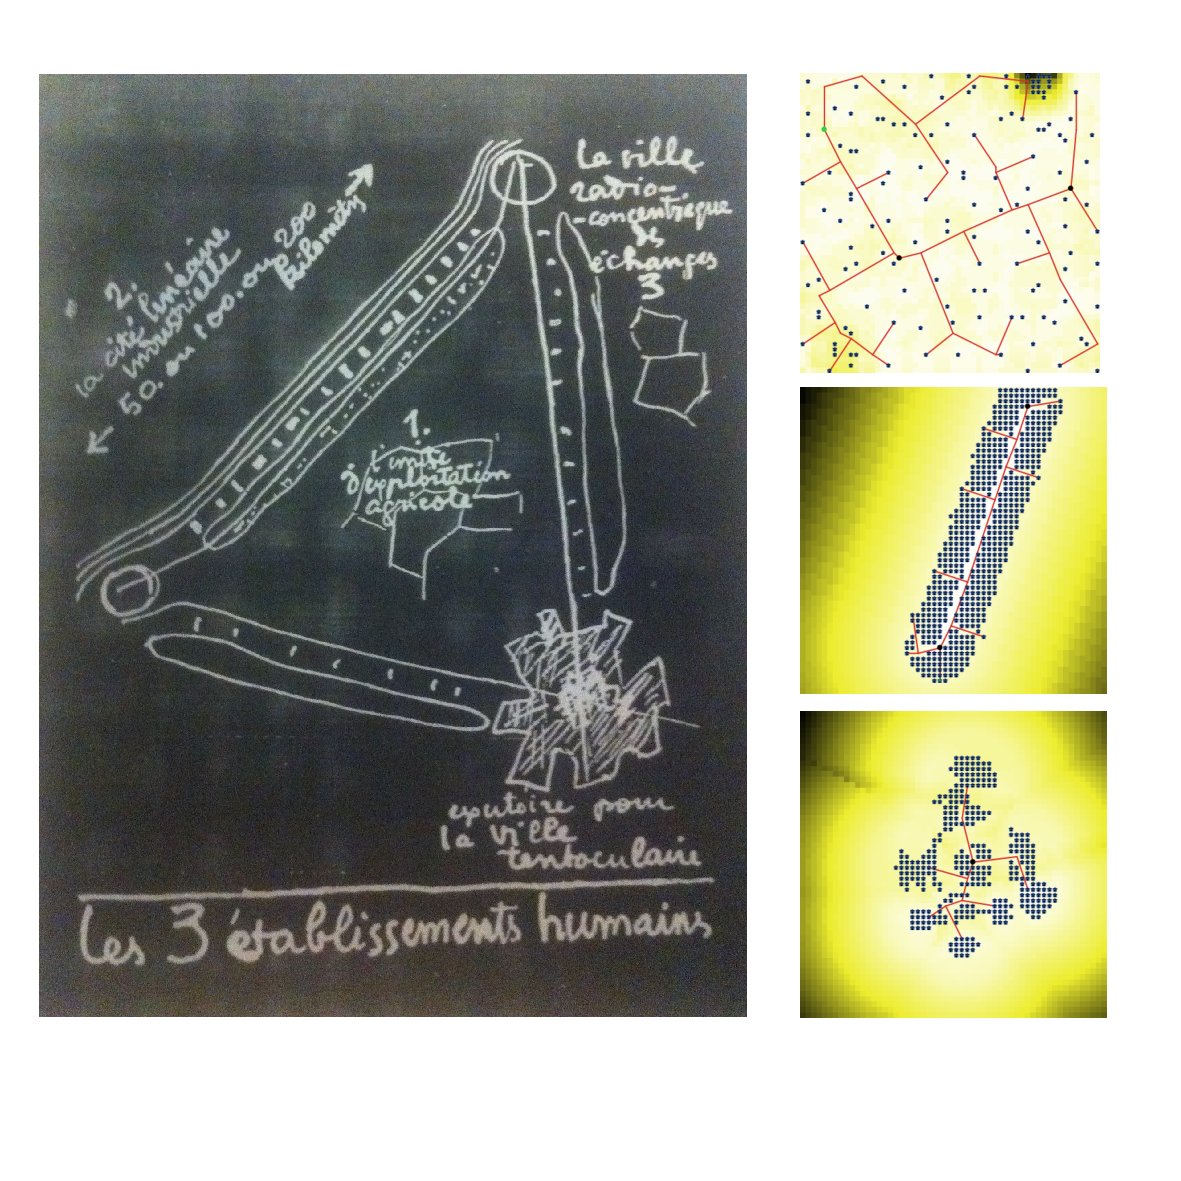
\includegraphics[trim=1cm 3cm 0.5cm 0cm,width=0.45\textwidth]{figures/corbu}
\caption{Typical patterns reproduce \noun{ Le Corbusier} analysis of ``human settlements'' When trying to theorize urban planning by first analyzing ``by hand''
the form of cities, \noun{ Le Corbusier}
has enlighten 3 types of settlements, that are radio-concentric cities,
linear cities along communication roads and the rural settlements.
We were able to reproduce this typology by playing with values of
weights (first only $d_{1}=1$, second only $d_{2}=1$ and third $d_{1}$and
$d_{3}$ of equal weights). Source of drawing: \cite{mangin2004ville} }

\label{fig2}

\end{figure}




\paragraph{Typical patterns}

We launch the model on random initial configurations, with randomly
distributed centers whose activities are also random but are globally
balanced between all possible activities. The initial network is created
through progressive connexion of connected components (what always
terminates since the number of connected components in the network
is then strictly decreasing). Different configurations of the weights
allow to generate very different structures. The obtained patterns
for extreme values of parameters (e. g. with only influence of density
on values, or of distance to centers) were quite the one expected
as there is in such case less emergent behavior. It is striking to
note that some characteristic patterns exactly correspond to the structures
that \noun{Le Corbusier} has analyzed when trying to build a typology
of the \textit{3 \'Etablissements humains}\textit{\small{} }(human settlements)
as it is summed up by \noun{Mangin} in \cite{mangin2004ville} (see
figure 2 for details).


\paragraph{Classification of structures}

Thanks to the morphological indicators, we were able to proceed to
a description of morphological classes that can be obtained with any
values of the parameters. The projection of a configuration in the
plan $Vect(D(t_{f}),M(t_{f}))$ allows to understand how the structure
are different and where they are situated in a certain ``classification''.
Fig. 3 sums up the results of that classification.




\begin{figure}[htp]
\centering


\subfloat[Projection in the plan and
some structures associated to some particular points. Three type of
structures are very close and may sometimes not be distinguish through
our simple indicators. The area close to zero corresponds to ``unfinished''
growth, that is structures that occupy only a small part of the world,
that does not allow to compare directly with structure of bigger
magnitude.]{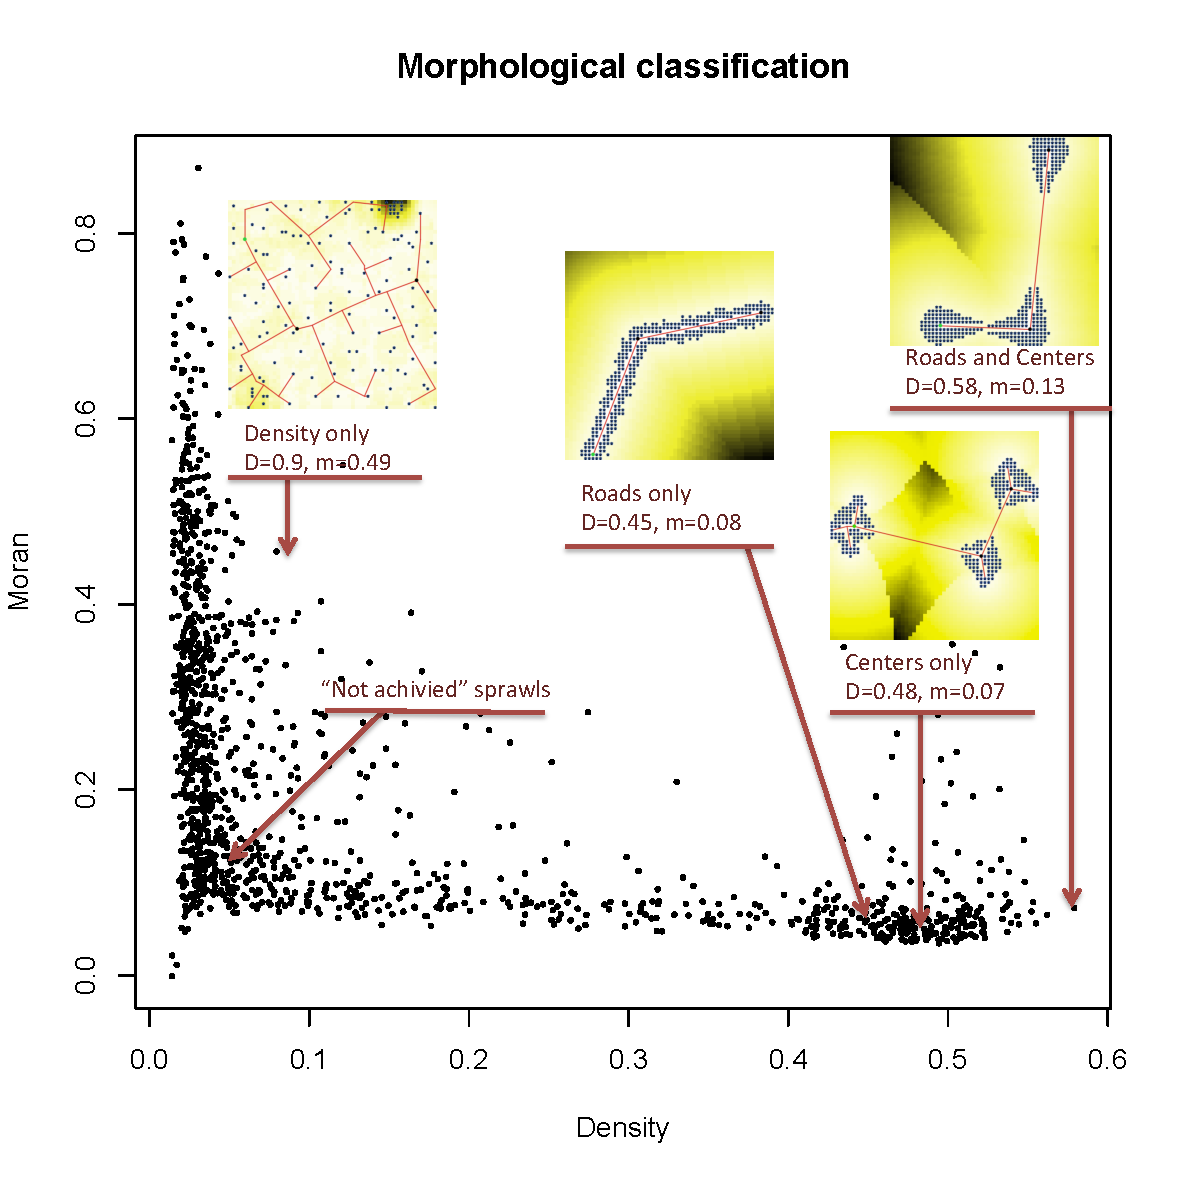
\includegraphics[width=0.45\textwidth]{figures/morpho}}\hfill{}
\subfloat[Influence of each parameter
on the location of the structure in the morphological plane. Color
darkness correspond to the relative weight of the parameter in each
case. If the previous plot showed that extreme cases were located
at expected places, this one shows that dark point are quite uniformly
distributed for the role of centers, accessibility and roads. That
means that some combinations created some ``chaos'' in the location
of structures. Only density weight gives one predictable result: the
fact that the cloud of points in low densities corresponds to great
influence of density in growth. However, the could at the right of
the plot shows that interaction between weights quickly limits that
predictability.]{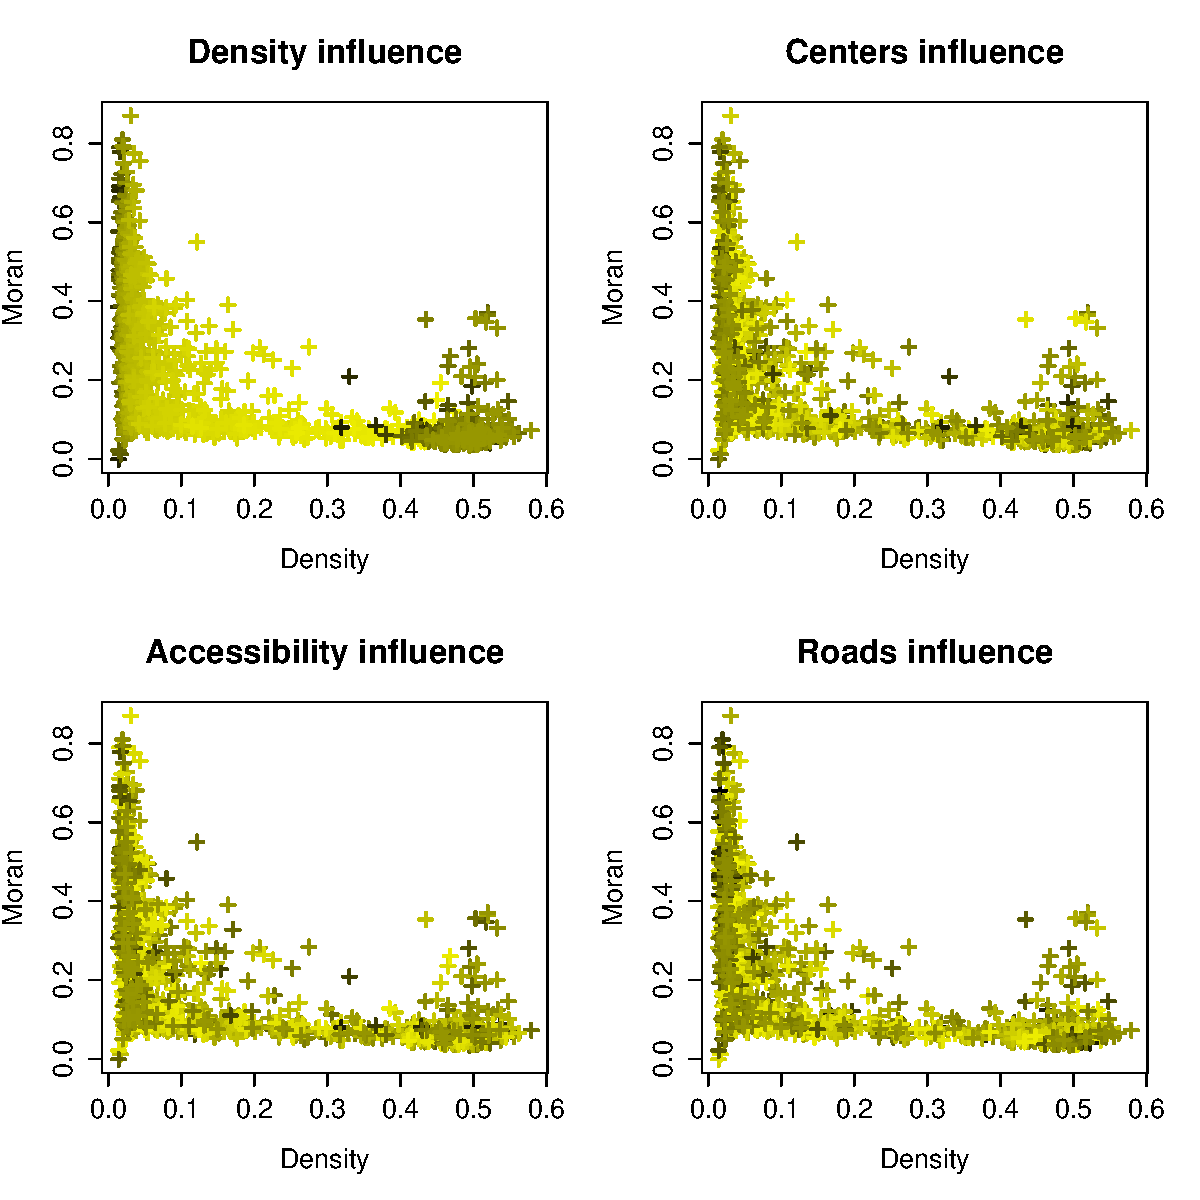
\includegraphics[width=0.45\textwidth]{figures/paramInfluences}}

\caption{Morphological classification of structures.}

\label{fig3}

\end{figure}



For extreme values of parameters, the results were quite the one expected,
but some combinations seem to project the structures at unexpected
places, what we can take as a sort of emerging chaos in the global
system.


\subsection{Sensitivity analysis and exploration of the parameter
  space : internal validation}



\begin{figure}[htp]
\centering
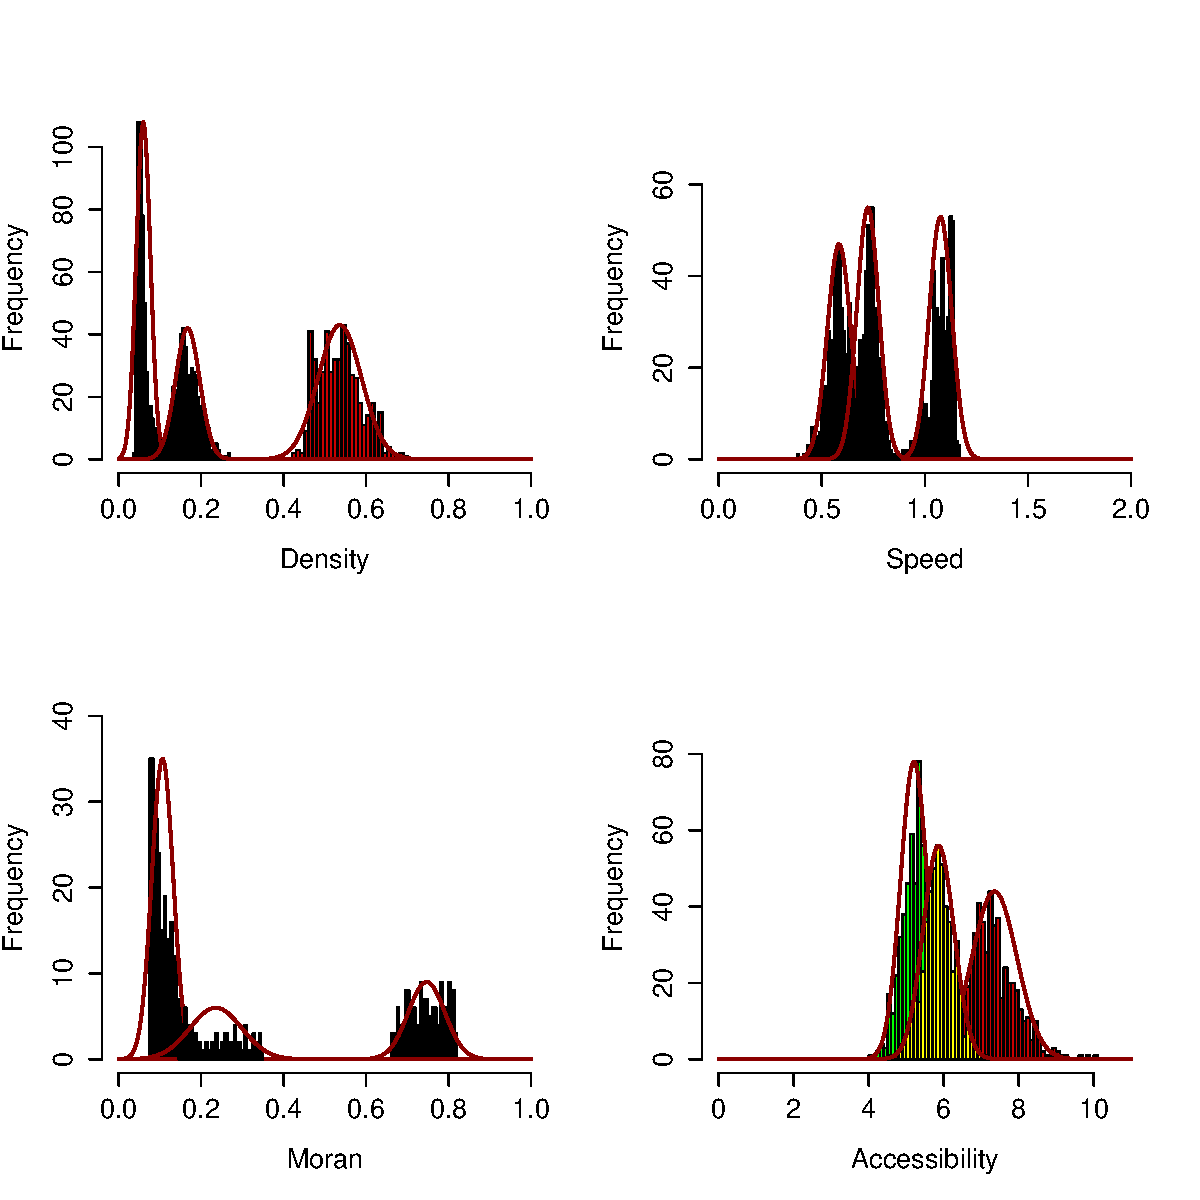
\includegraphics[width=0.45\textwidth]{figures/manyConfs}
\caption{Statistical distribution of outputs
for sample points in the parameter space . For many
combination of weights $(c_{k})$, we calculated the distribution
of these 4 outputs on around 500 repetitions for random initial configurations.
We represent for each output three points of the parameter space that
give quite disjoint distributions, to show how we are in those case
able to compare them and draw conclusions from the comparison. At
each time, we plot the Gaussian fit (red curves), that is generally
close to the distribution. The shape of distributions translates the
small sensitivity of the model to spatial configuration, since it
covers at most one tenth of the range of output functions (0.1/1 for
density, 1/10 for accessibility e. g.). That confirms the consistency
of the model since we expected the output to be quite independent
of initial positions and that their comparison could lead to statistically
consistent results. That allows also to fix the number of repetition
needed to obtain a certain level of statistical significance in the
outputs of the model : for example, under assumption of normal
distribution for an indicator and its mean, with $\sigma = 0.2$ supposed constant and estimated, we need $n=\frac{2\sigma\cdot 1.96 }{0.1}^{2}\simeq60 $  repetitions to have a 95\% confidence interval of length 0.1 on the calculated mean.}

\label{fig4}

\end{figure}



\paragraph{Sensitivity to initial conditions}

To determine the magnitude of repetitions useful to get meaningful
values of output functions and to ensure some validity in the results,
it is necessary to investigate the sensitivity of the model to initial
conditions of the spatial configuration. Indeed, if the conclusions
that can be drawn in a particular case are significantly modified
by small changes in the spatial configuration, one will differently
apply the model than in a case where abstract topology of activities
has more influence: one will obviously elaborate totally different
exploration heuristics to proceed to optimisation.

Therefore, we launched large number of simulations with same parameter
values but different initial configurations, in order to get statistical
distributions of outputs at fixed parameters. Standard deviations
were calculated for samples of the parameter space (around 20 samples)
and the distributions were each time of same amplitude and same deviation.
Fig. 4 shows these distributions for the sample corresponding to equal
weights to each parameter. Given the numerical values of deviations
(each time around 0.1 times the amplitude of the function), we can
conclude that outputs are significantly less sensitive to spatial
positions than to topology of activities and parameters values (as
the exploration of parameter space results show in the following).
That justify the small number of repetition needed to have reasonable
values.



\begin{figure}[htp]
\centering
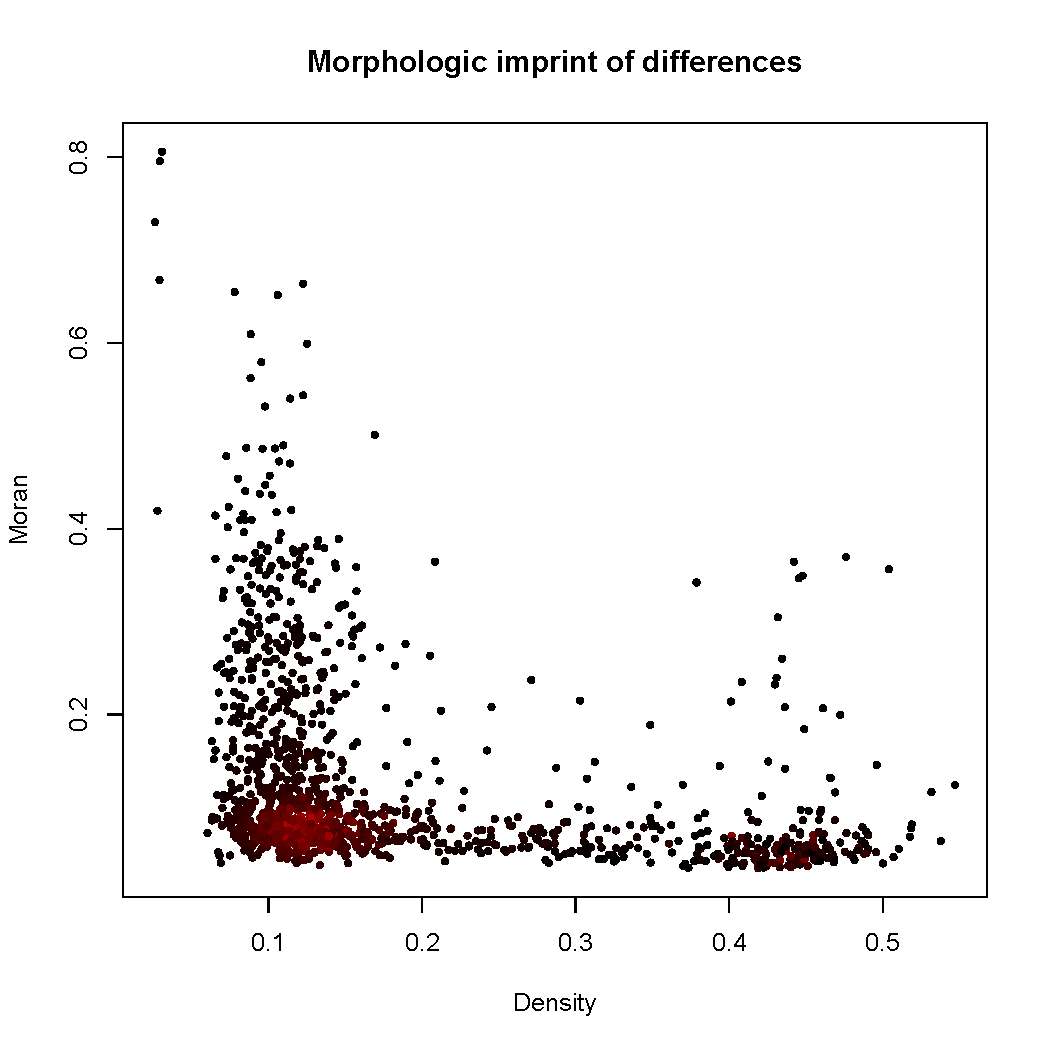
\includegraphics[width=0.45\textwidth]{figures/diffImprint}
\caption{Morphological projection of symmetric
differences between configurations for both update types.
Each point corresponds to many realizations (50) for a given value
of parameters. Each time, both structures for continuous ($N=1$)
and sequential ($N=20$) are generated, symmetric difference is computed
and projected in the morphologic plan. Points are colored according
to their ``significance'', defined by the product of local density
of points in the cloud (closely clustered points correspond to more
frequent configurations) by the relative size of the configuration
(large configurations correspond to large difference and are therefore
more significant). The wide spread shows a strong sensitivity. An
other plot of superposed imprints for each type of update showed quite
disjoint sets, what confirms this sensitivity. It is however relativized
by the concentration here of significant points, which means that
side effects are ``constant''. Therefore taking a compromise between
two types of updates should give stable and reasonable results.}

\label{fig5}

\end{figure}



\paragraph{Sensitivity to update type}

The generated structures seem to be quite sensible to the type of
update that is done at each time step, i. e. to the number of cells
that are built at each time step. That comes from the fact that at
each time step, houses are built simultaneously without update of
patches values. It is a consistent view since real value functions
should have a certain response time that we can suppose of the magnitude
of $\tau$. However this paradigm can be limited and it is necessary
to find a compromise value for $N$ that leads to reasonable configurations.
We can explore a grid of the main parameter space (weights of variables)
and at each time generate patterns corresponding to a ``continuous''
update ($N=1$) and a ``sequential'' one ($N=20$ in our case),
calculate the symmetric difference $\mathcal{D}=\{(i,j)|\delta^{cont}(i,j,t_{f}^{cont})\neq0\}\Delta\{(i,j)|\delta^{seq}(i,j,t_{f}^{seq})\neq0\}$,
and plot the corresponding sets in the morphological plan. Results
are shown in figure 5, including a colored representation of significance
of points. We conclude that the model is highly sensitive, but that
bord-effect stay the same so finding a good compromise by experience
(giving ``consistent'' structure) should solve the problem.


\begin{figure}[htp]
\centering
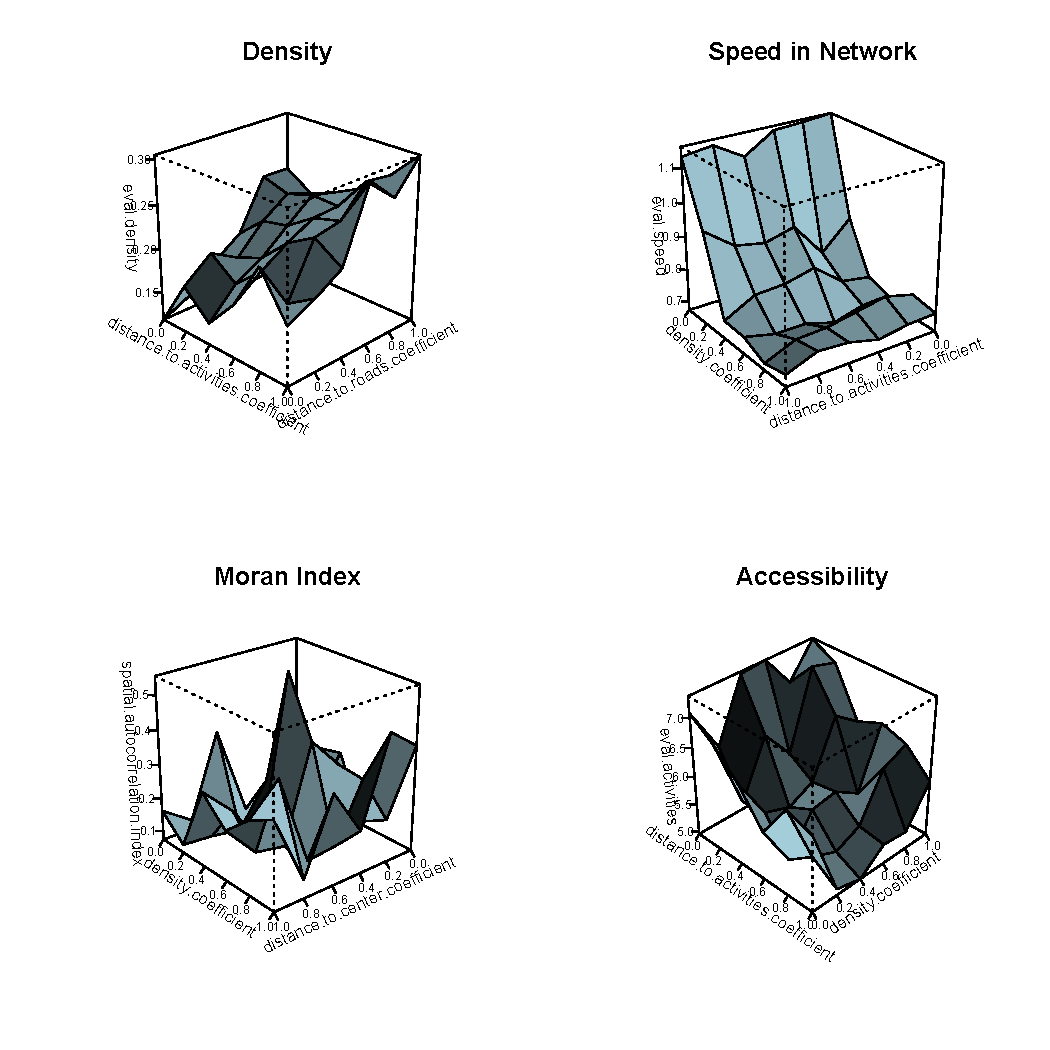
\includegraphics[width=0.45\textwidth]{figures/plots3d}
\caption{Surface of evaluation functions depending
on two parameters. We chose some combinations of parameters
that seemed to be interesting. We can extract the ranges of outputs
and observe their regularities. The chaotic behavior of Moran index
and accessibility confirm the existence of chaotic mechanisms in the
system. Speed appears to be regular, what implies that network spread
is not so far from linear regarding these parameters. Other combinations
gave chaotic behavior.}

\label{fig6}

\end{figure}


\paragraph{Exploration of the parameter space}

We explored a grid of the 4-dimensional space of the ``main'' parameters,
the relative weights of variables, to evaluate the global behavior
of outputs when parameters vary. Other parameters such as $r$ or
$d_{s}$ were not included in the exploration because they have real
proxy that we can reasonably fix (around 5 cells seemed in general
to generate the structures closer to the real world, what is significant
whatever the scale of application, as the size of a district, it gives
50m, characteristic size of blocs, of the city 500m size of a district
and of the system of cities 5km characteristic distance between cities).
Step was 0.2 for each parameters, with 5 repetitions for each combinations,
what lead to the calculation of around 3200 configurations. Examples
of surfaces defined on the space of two parameters are shown in figure
6. For each measure, we chose to plot against 2 parameters out of
the 4 possible dimensions, whose were supposed to have more influence
and for which the surfaces were the most revealing. Economic evaluation
was not plotted for efficiency reasons. However, since it depends
directly on morphology and network and that it is not probable that
the function would exactly smooth the irregularities, we can conclude
that the shape of its surface would present same patterns of irregularity.
The exploration allows first to appreciate the regularity of the outputs,
what is essential to understand the internal mechanisms of the model
that appear in some point as being somehow chaotic and non-linear.
Secondly, it gives the range of outputs, allowing to state the robustness
regarding initial conditions as we stand before.


\subsection{Concrete application}

Since we have shown that outputs on which we want to optimize, such
as accessibility to activities or network performance, are significantly
more sensible to initial configuration of activities than to spatial
distribution, we can apply the model to the optimization of activities
repartition, given an existing spatial structure. That situation can
occur in a planning problem, then one has to decide possible land-uses
of predefined zones.

The concrete situation will consist on the planning from scratch of
a new district, where attribution of activities to areas has to be
determined (2 types of activities, residential or tertiary). Transportation
infrastructure is already implanted and the station will act as center
with a fixed third activity. For each area, centroid is a center and
the initial network consists on main roads existing on the empty district.
Configuration is imported from GIS shapefile so the application can
be done on other cases, as soon as one has required files (see S2).
The real world situation is the district of Massy Atlantis, France,
which have just been built and planned (2012) and for which we would
like to study if a more optimal planning may have been done. We fix
a value of parameters translating the situation, that is : high influence
of activities ($c_{4}=1$) because agents will want to have accessible
home, workplace and station; medium influence of density ($c_{1}=0.7$)
because the houses have to fill reasonably the available areas; no
influence fo roads since we suppose that the initial network is already
built and has a few influence because of the scale; and no influence
of centers because centers are here abstract entities representing
a all area. We then launch the calculation of configuration for all
possibilities of distribution of activities in the areas (exponential
on the number of free centers, 510 calculations in our case, what
gives around 2500 runs with repetitions) and plot configuration in
the plan of economic performance and accessibility (most significant
fitness functions in our case). Results are shown in figure 7.




\begin{figure}[htp]
\centering

\subfloat[Left: existing masterplan
for the district as it has been realized. Areas correspond to colored
zones, and actual activities correspond to the color. Station, not
mentioned is in the upper left (see center positions in model); Right:
example of obtained configuration, color correspond to possible distribution
of activities.]{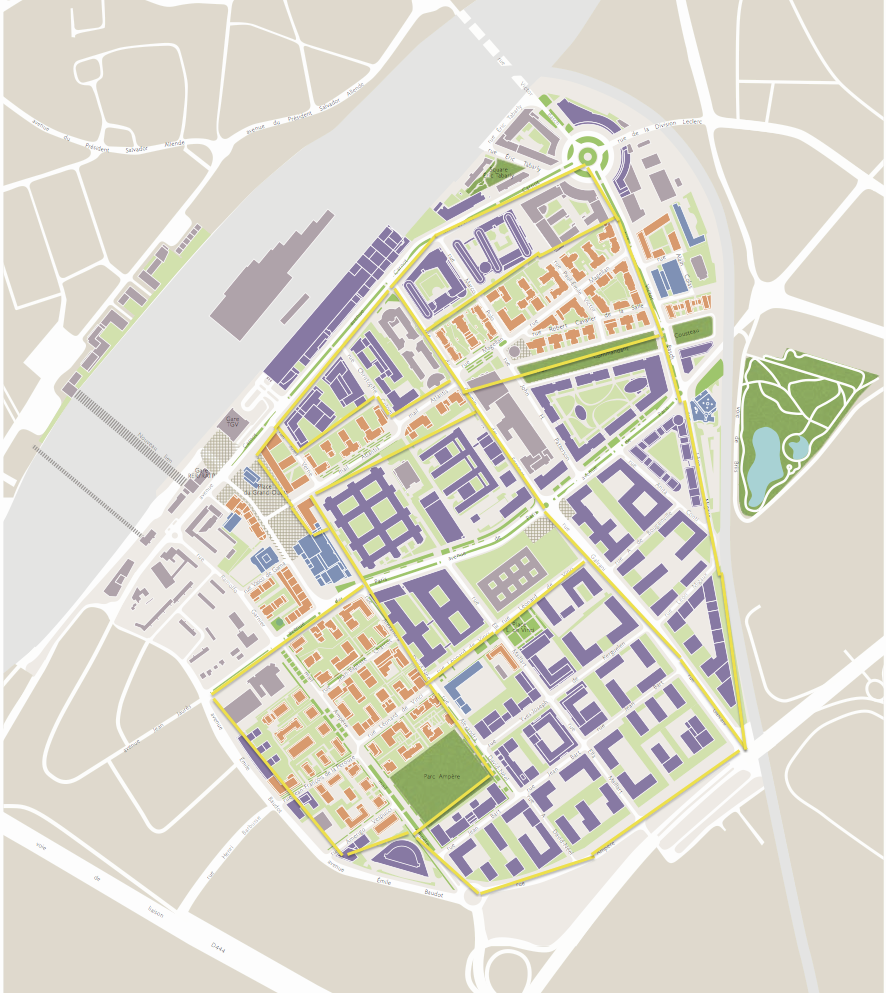
\includegraphics[width=0.21\textwidth]{figures/Atlantis}\hfill{}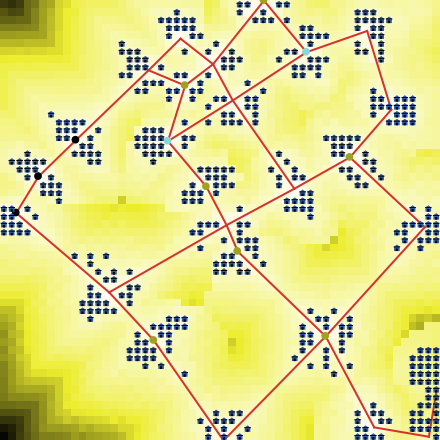
\includegraphics[width=0.23\textwidth]{figures/example}
}\hfill{}
\subfloat[Pareto plot of configuration
in the plan economic performance/accessibility. Green point corresponds
to the real situation, that is in fact not so far from the Pareto
frontier so is a mean solution in quality ($E=0.07$,$A=0.76$). Red
points that are some of the Pareto-optimal solutions with a good compromise
between the two objectives, correspond to situation where activities
are totally mixed.]{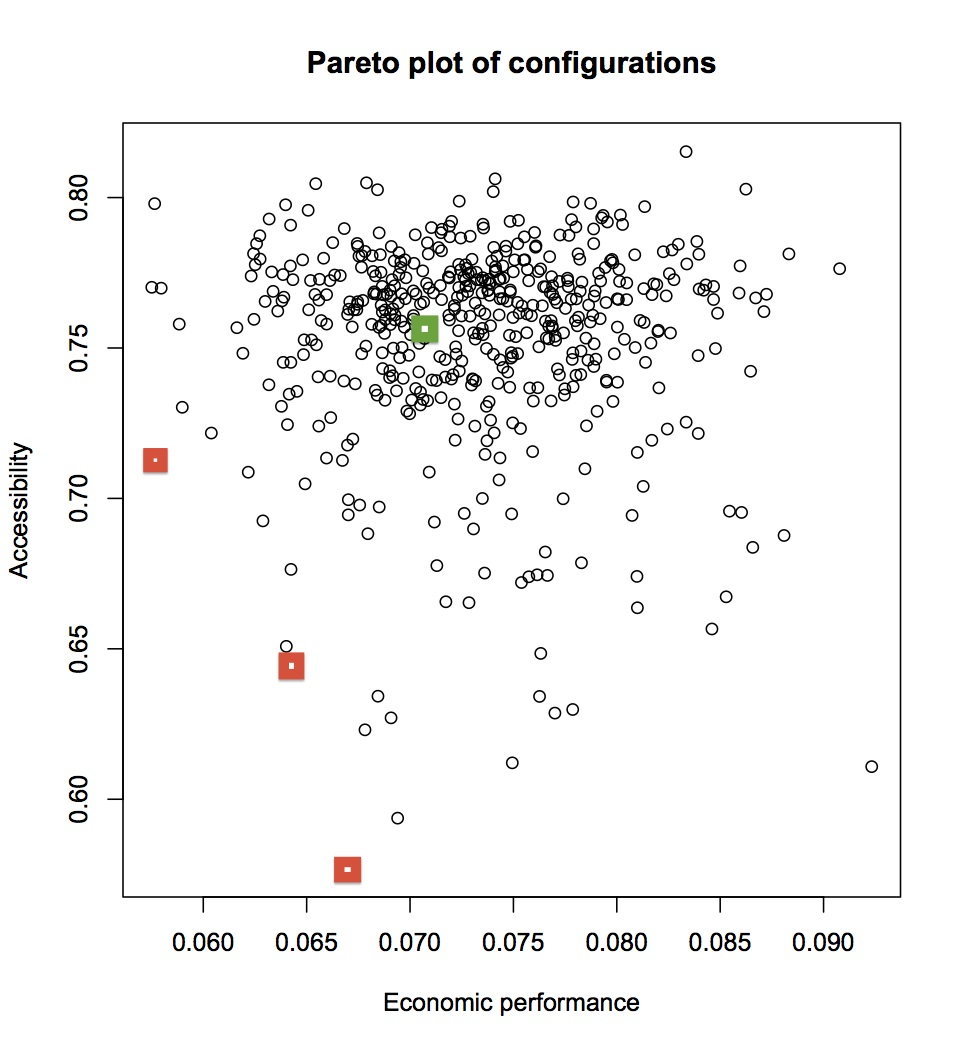
\includegraphics[width=0.45\textwidth]{figures/applicationcorrect.jpg}
}

\caption{Concrete application.}

\label{fig7}

\end{figure}



We plot the configuration in the plan corresponding to the two objectives
and we naturally obtain a Pareto-front of ``optimal solutions''.
We observe that the real configuration is not so far to be optimal;
although it favors more accessibility than economic performance.
By examining two optimal points that are good compromises, we see
that the corresponding combinations of activities are one where they
are maximally mixed (totally heterogeneous repartition). That is an
interesting fact and may be a clue towards evidences for more mixed
land-uses in planning. We conclude that the application is efficient,
since it allows to propose an optimal planning regarding these criteria
in such a situation. It could be generically used by planners in similar
situations (staying very careful on the conditions of application).


\section{Discussion}

The reproduction of existing urban facts (in the sense of the morphological
structures) and the possible applications showed that the implemented
model may be useful for evidence-based decision-making in urban planning.
However, many aspects can be discussed as they raise crucial questions
and would need further explorations.




\paragraph{Scale of the model}

One ambiguity of the model is that it can be applied at several scales
and that its agents have not necessary correspondence in the real
world. Indeed, as we saw in results and applications, it can be used
at the macro scale of a system of cities (settlement patterns), the
meso scale of the city (patterns for one city) or the micro scale
of the district (concrete application). Without going into an ontological
debate on the quantity of abstraction of object, it can obviously
be pointed as a huge issue. However, we argue that this multi-scale
application is legitimate. First, a large number of urban systems
and associated processes have been shown to be scale-free as \noun{Pumain}
shows in \cite{pumain2004scaling}, what implies that scaling laws
can be present in our model and that it is therefore appliable at
any scale, since qualitative properties should remained unchanged
(quantitative evolution of relations should depend on the underlying
exponents of the scaling laws). Furthermore, urban form have been qualified to have fractal
properties (\cite{FractalCities}) what would strengthen that paradigm.
Following \noun{Barthelemy} in \cite{2013arXiv1309.3961L} when he
insists on the fact that the failure of most multi-agent urban models
is that they don't focus on the ``dominating'' physical process but
integrate many aspect that have in reality no influence on the emergent
properties of the system, we suppose here to have isolated at least
``good'' proxies of dominating processes.

\bigskip{}



\paragraph{Local application}

When the model is considered at a meso or micro scale, one could object
that it neglects too much phenomena such as economic exchanges by
considering the system as a ``closed'' system (it is formally closed
but not ``closed in reality'', since just the new constructions
can be seen as exchanges with the outside - the precise critical would
be that in and out flows are too much simplified). As economic models
considering the global complex network of cities such as in \cite{andersson2003urban}
have also reproduced well existing patterns in urban systems, it is
obvious that the equivalence of approaches and the compromise that
need to be made in each case have to be further investigated. It joins
the fundamental issue, already implicitly raised in the previous
point, of the existence of a minimal dimension for a generalized representation
of urban systems. Concretely in our case, attractivity of centers
is a proxy for economic processes, and although the model does not
directly include economic considerations, they are underlying, confirming
that urban processes are strongly interdependent. The problem would
be to understand how general the dependance is and if a generalized
minimalist formulation can be constructed. Speculations towards that
have been proposed by \noun{Haken} in \cite{haken2003face} with the
notion of semantic information that would be linked to properties
of attractors of dynamical systems. This theory has however neither
been quantified, confirmed or invalidated.

\bigskip{}



\paragraph{Quantitative calibration}

The question of validity of the model is also linked to the need for
a fine quantitative calibration on real patterns. Calibration of such
models is still an issue, since on the one hand calibration on errors
on proxies for output function does not directly influence the spatial
patterns but on the other hand calibration on spatial patterns is
too constraining because it eludes ``similar'' patterns. Some work
has been done on tries for such calibrations such as in \cite{maria2003stochastic}
but the results are not satisfying. To go in that direction, we would
first need to apply the model with finer grain for the spatial resolution,
i. e. on a very large world. Computational issues can appear, even
though we optimized processes in the implementation (see supplementary
material S2, e. g. single calculation and caching of network shortest
paths allow a huge gain in computational complexity). But the increase
in size can also cause methodological issues, since the amount of
details in patterns can become too huge and bring more noise in the
indicators, biasing the results. Therefore, an additional operation
could be a solution, that is the extraction of the morphological envelope
of the generated pattern, following the innovative method proposed
in \cite{tannier:halshs-00461657,frankhauser2005multi}. Other ways
to deal with noise such as gaussian smooth should also be investigated.

\bigskip{}



\paragraph{Complex coupling with economic model}

The way we proceed to economic evaluation consists in a simple coupling
with an other agent-based model. It could be a direction of research
to look towards a complex coupling (in the sense of \noun{Varenne}
in \cite{varenne2013modeliser}) between the two models. Indeed, considering
the sprawl at an other time scale implies simultaneous evolution of
inhabitants, rents of buildings and values of terrain. Of course such
a coupling would lead to a completely different model that would need
to be explored again and that would be appliable to totally different
situations (as evaluation of long-term rent policies for social diversity
for example).

\bigskip{}



\section{Conclusion}

We have proposed and explored an heterogeneous CA model to simulate
urban growth patterns, using also a new way to evaluate economic properties
of spatial patterns. It has shown to be able to reproduce characteristic
urban facts of a possible typology of ``human settlements'' (cf
3.1). Furthermore the model was applicable to a concrete situation
giving an ``optimal'' (in the Pareto sense) solution to a planning
problem in a zoning context. The results go in the direction of evidences
for a ``mixed-use'' city, on which literature is still poor and
that could be the object of future work. That paradigm is proposed
by urbanists such as \noun{Mangin} in \cite{mangin2004ville} (concept
of the ``passing city'') and would need to be confirmed by quantitative
results.

Beyond these technical facts useful for planning purposes, we argue
that our work gives a vision of the current state ``quantitative
urbanism'', confirming the view of \noun{Portugali} in \cite{portugali2012complexity},
in the sense that the conception and application of such models is
in fact very subtile and can lead to many misunderstanding and contradictory
results. Here the link between model and application is in that frame,
and can become obviously wrong just by an application with other parameters.
However, we stand that a better quantitative comprehension of urban
systems begins to be actual and that evidence-based solution to planning
problems are real, at the opposite of the vision of \noun{Lefebvre}
in \cite{henri1968droit} when he stood that scientific approaches
could never translate or predict the mechanisms of a city.


\bibliographystyle{unsrt}
\bibliography{biblio/projetCSMS,biblio/global,biblio/ccupd}



\section*{Appendices}

\subsection*{Appendix A : Description of the agent-based model for economic evaluation}

\subsubsection*{Purpose of use}

We want to propose a model similar in behavior to \noun{Schelling}'s
segregation model (\cite{schelling1969models}), based on the work
by \noun{Benenson} on residential dynamics (\cite{benenson1998multi}).
The question of the influence of the underlying spatial structure
on the output of the model appears as crucial. \noun{Banos} showed
in \cite{banos2012network}, unlike previous results, that the network
structure add strong effects on the convergence speed of the model
and on the final result.

Therefore, our approach is to proceed to a simple coupling that consists
in evaluating the spatial structure by measures on the final configuration
given by the dynamical economic agent-based model. We are able to
define a ``segregation potential'', in the sense of the segregation
induced by the spatial structure embedded in a \noun{Schelling}'s model.


\subsubsection*{Description of the model}

We are still located in the lattice world, in which cells values,
houses positions and network are fixed.

A new variable is associated to houses (i. e. occupied cells), which
is the rent $r(i,j,t)$. Mobile agents are households $h_{k}\in H$
that have a wealth function $w(k,t)$ and occupy the house $(i(k),j(k))$.

We begin with no occupied house, initial rents are a mean value $m$.

At each time step:
\begin{itemize}
\item Already present households may decide to move to an other inoccupied
house, depending on the condition $\frac{v(i(k),j(k))}{v_{max}}\cdot\frac{w(k,t)-r(i(k),j(k),t)}{max_{k}(w(k,t)-r(i(k),j(k),t))}<\epsilon$,
where $\epsilon$ is a threshold parameter fixed. They occupy the better
house possible according to $\frac{v}{r}$. If no house is available,
they die (leave the city)
\item $N_{i}$ new immigrant come, with a random wealth $w\sim\mathcal{N}(m,\sigma)$
with $\sigma$ parameter small regarding $m$, and occupy best free
houses (maximal number of immigrant is fixed by available houses).
\item Rents are updated, set to the mean within a given radius $r_{e}$
of wealth of households and rents of surrounding houses (gentrification
effect).
\item Wealth are not updated considering the supposed small time scale.
\end{itemize}





\begin{figure*}[htp]
\centering

\subfloat[Time-series of rents.]{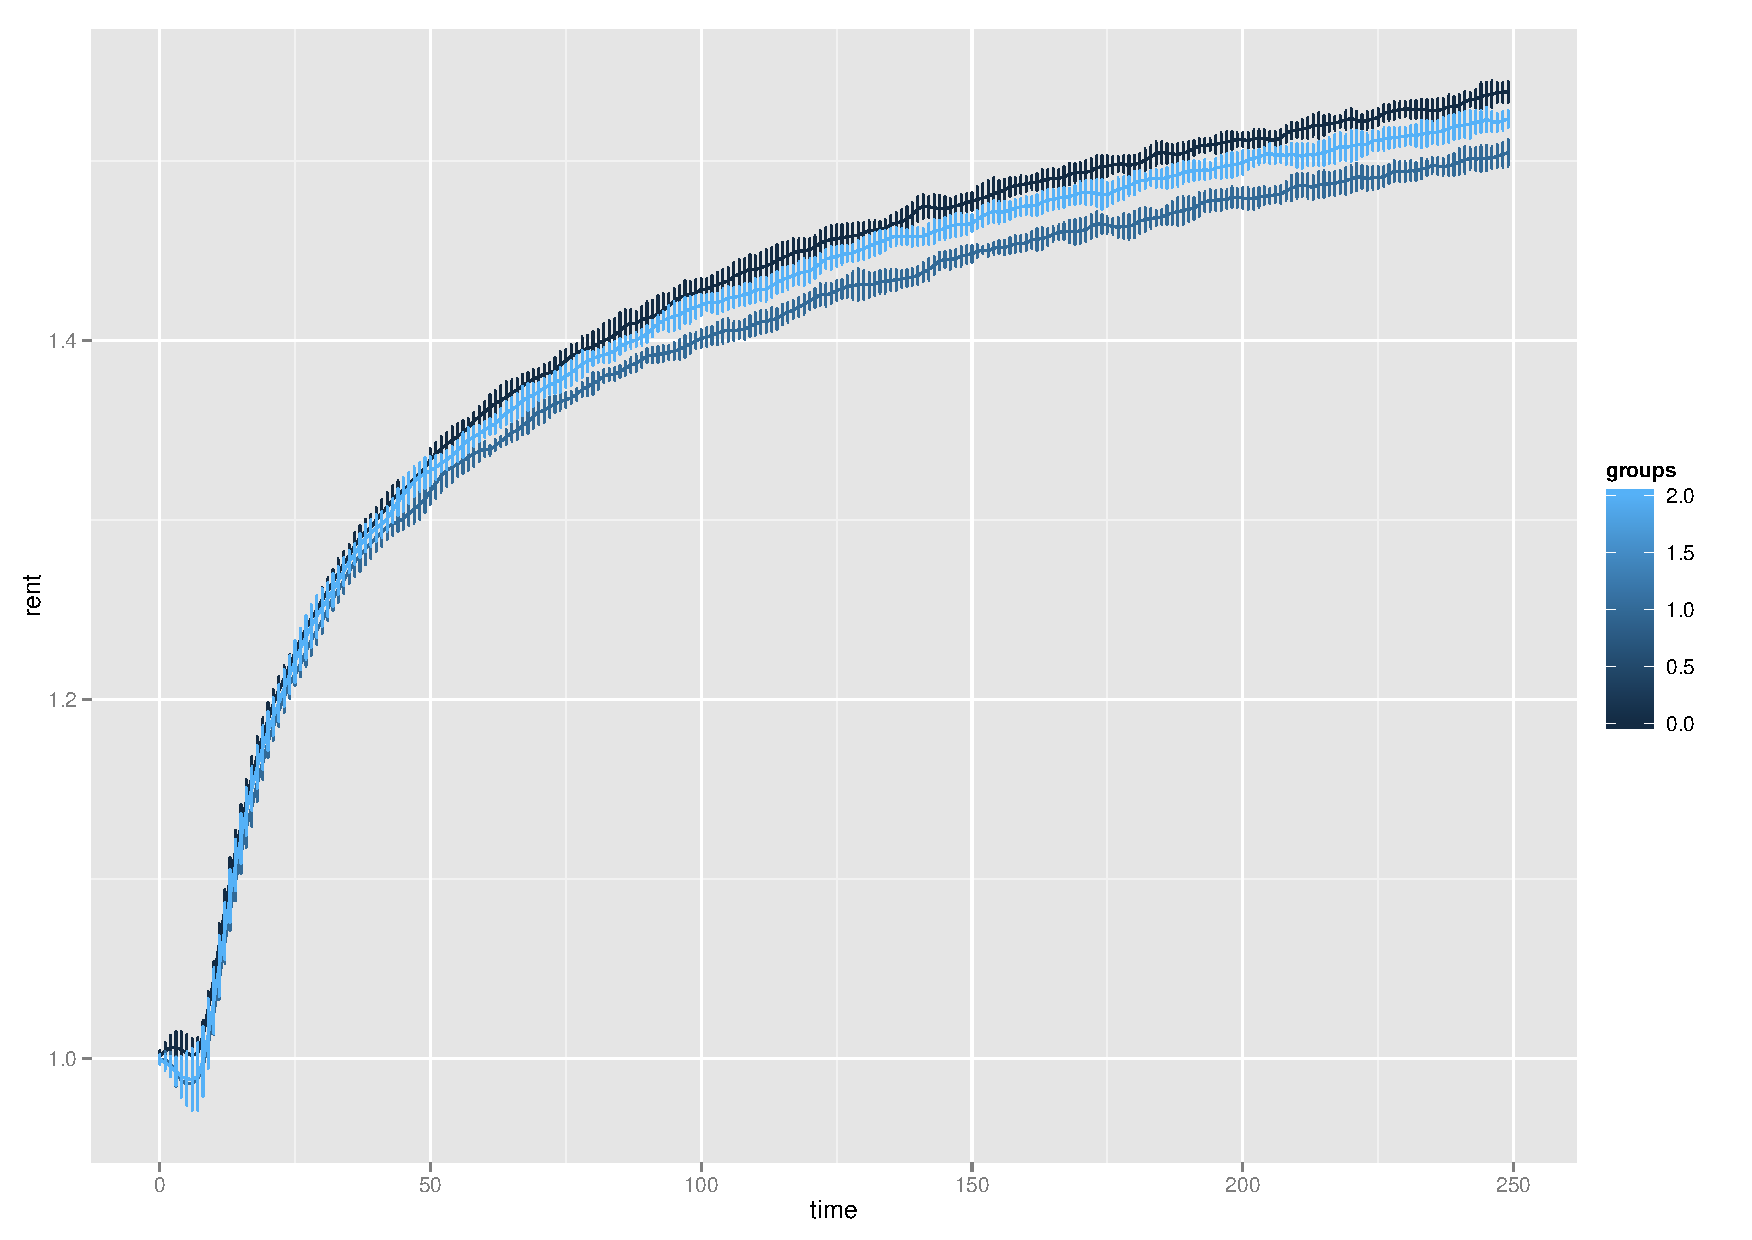
\includegraphics[width=0.45\textwidth]{figures/convergenceRents}}\hfill{}
\subfloat[Time-series of segregation indexes.]{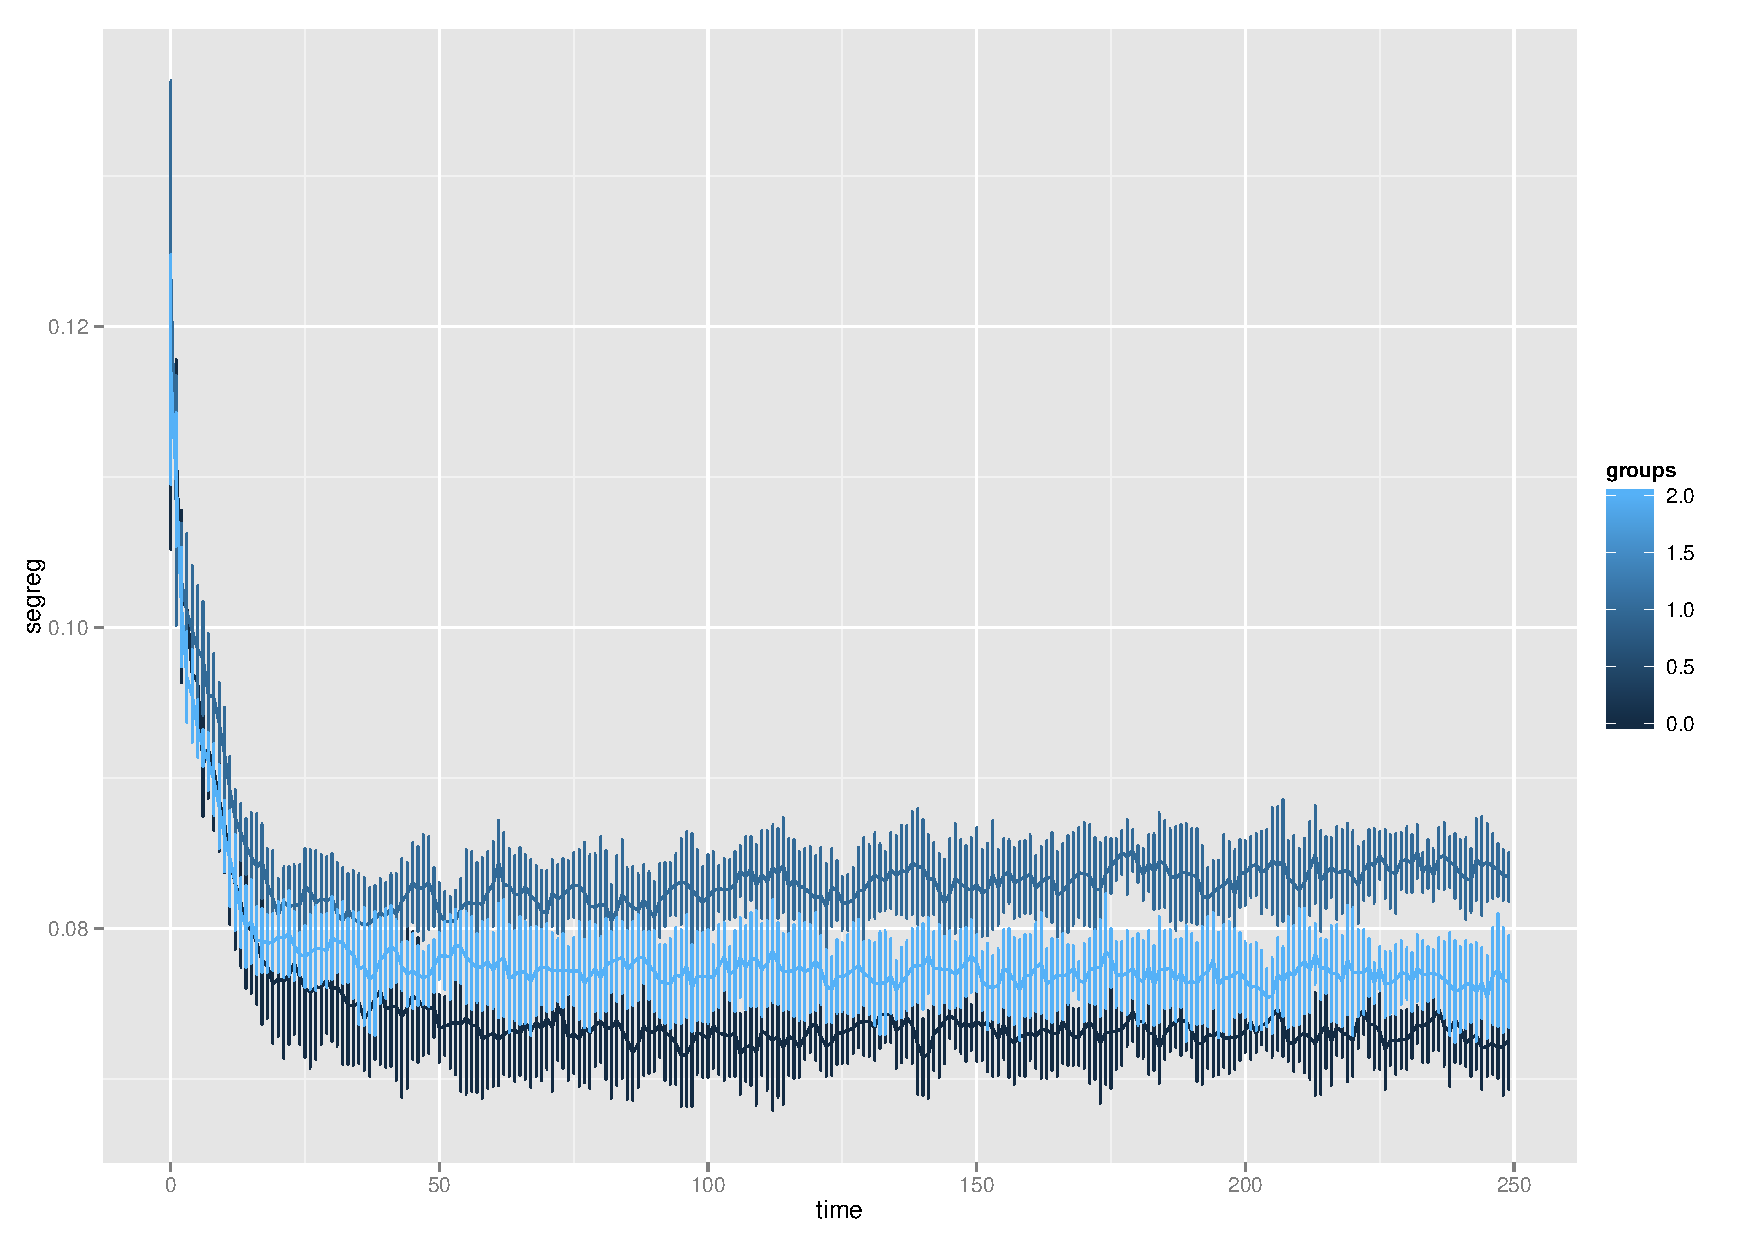
\includegraphics[width=0.45\textwidth]{figures/ConvergenceSegreg}
}

\caption{Convergence of the model. For each plot, each three curves correspond
to a configuration of parameters. The values are calculated on 20
repetitions of the economic ABM, and the calculation is repeated on
100 initial spatial configuration, for which the error bars of distribution
are plotted for each point.}

\label{fig8}

\end{figure*}



\subsubsection*{Convergence and evaluation of segregation}

After a certain number of time steps (around 100 in practice) the
system freezes concerning indicators of cumulated wealth and segregation
index, as it is explained in the literature. Figure 1 shows the convergence
of segregation index and mean rent of houses on many repetitions of
the model for different values of parameters.

We are then able to calculate the segregation index on the frozen
state, and defined by the classic spatial diversity index calculated
on households:
\[
d=\frac{1}{2max_{h}(w(h))}\cdot\frac{\sum_{h'\neq h}\frac{\left|w(h)-w(h')\right|}{d(h,h')}}{\sum_{h'\neq h}\frac{1}{d(h,h')}}
\]


\bigskip{}
\bigskip{}

\subsection*{Appendix B : Source code of the implementation of the model}

Core source code of the NetLogo implementation of the model, sample
of data used for applications and source code for generation of plots
and charts are available online at
http://github.com/JusteRaimbault/Project.


\end{document}
